The gearbox meshing system~\cite{chen2014motor} analyses the impact force and meshing time in a motor-transmission drive system,
where a shift actuator is used to switch between gears.
%
Depending on the angular position with which the sleeve arrives at the gear, impacts may occur which can delay the meshing process.
%
The analysis goal in this case is to find the worst-case accumulated impact impulse, as well as the longest meshing time.


\begin{figure}[t]
\centerline{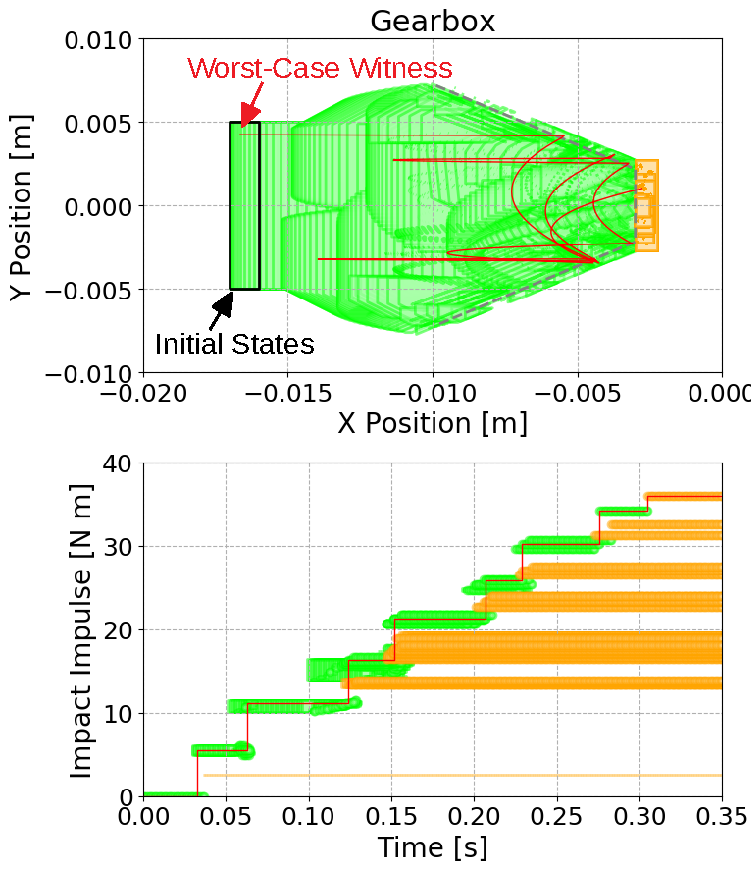
\includegraphics[width=0.8\columnwidth]{images/gearbox_annotated}}
\caption{The reachable set for the gearbox system is shown on the x/y plane (top), as well as the total impact impulse over time (bottom).
%
The red line shows a worst-case witness which bounces seven times and reaches the maximum impact before meshing.
%
A video of the reachability computation is online at \url{https://gofile.io/?c=haaCmh}, and a video of the worst-case witness
simulation available at \url{https://gofile.io/?c=Gd5N2B}.}
\label{fig:gearbox_reach}
\end{figure}

\begin{figure}[t]
\centerline{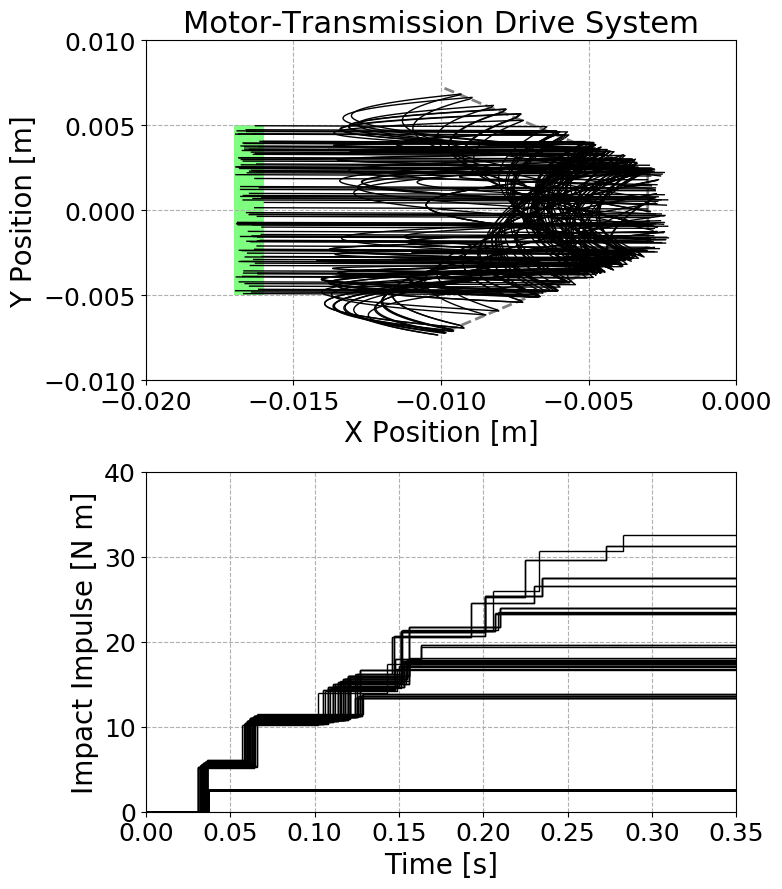
\includegraphics[width=0.8\columnwidth]{images/gearbox_sim.png}}
\caption{One hundred random simulations are shown for the gearbox system on the x/y plane (top), as well as the total impact impulse over time (bottom).
%
Notice the worst-case accumulated impact impulse from Figure~\ref{fig:gearbox_reach} was not observed in this simulation batch,
demonstrating that simulations can miss important system behaviors.
%
A video of the simulations is online at \url{https://gofile.io/?c=ypzXbv}.}
\label{fig:gearbox_sim}
\end{figure}
